\section{Topology}

A premise for implementing Paxos in the switch is that we also deploy
multiple switches to provide the necessary resilience to failures.
%
Thus we need to provision a switch topology.

In this section, we will present how we plan to achieve this.
%
Starting with a single switch, we show how it can use a controller to
shuttle packets between clients and services running on end-hosts (figure
\ref{figure:graph.single.switch}).
%
By linking three such switches together, one will typically want to install
Paxos middleware on each host to provide service replication and
fault-tolerance (figure \ref{figure:paxos.on.servers}).
%
We then propose that by moving Paxos from the hosts to the switches, one can
offer the guarantees of Paxos, \textit{transparently}, for a wide class of
services (figure \ref{figure:paxos.on.switches}).

Let us start with the simplest case: One switch.\index{Paxos!topology}

In figure \vref{figure:graph.single.switch}, a switch $S_1$ is connected to
several nodes through ports.  On one of these, the switch will receive
packets from a set of clients $c_1$, $c_2$, $\dots$, $c_n$.
%
It has an OpenFlow controller $C_1$ and three end-hosts $h_1$, $h_2$ and
$h_3$ running software to service client requests.

Note that the actual location of the clients is irrelevant to our current
discussion.  Our focus is on the possible merits of placing Paxos on the
switch, not on how clients are able to reach the services. We will therefore
\textit{assume} that we are able to communicate with a set set of clients on
a designated port.

\begin{figure}[H]
  \centering
  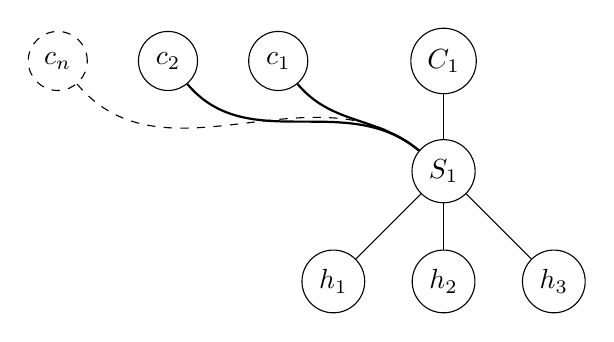
\begin{tikzpicture}[
      every node/.style={draw, circle, minimum width=0.75cm},
      x=0.7cm,
      y=0.7cm]
    \node (c1)    at (-3,  2) {$c_1$};
    \node (c2)    at (-5,  2) {$c_2$};
    \node [dashed] (cn) at (-7, 2) {$c_n$};

    \node (ctrl1) at ( 0,  2) {$C_1$};
    \node (S1)    at ( 0,  0) {$S_1$};
    \node (h1)    at (-2, -2) {$h_1$};
    \node (h2)    at ( 0, -2) {$h_2$};
    \node (h3)    at ( 2, -2) {$h_3$};

    \draw [thick] (c1) to[out=310,in=140] (S1);
    \draw [thick] (c2) to[out=310,in=140] (S1);
    \draw [dashed] (cn) to[out=310,in=140] (S1);

    \draw (S1) -- (ctrl1);
    \draw (S1) -- (h1);
    \draw (S1) -- (h2);
    \draw (S1) -- (h3);

  \end{tikzpicture}
  \caption{A single switch $S_1$ with its controller $C_1$, connected
    to end-hosts $h_1$, $h_2$, $h_3$ and clients $c_1$, $c_2$, $\dots$, $c_n$
    through ports.}
  \label{figure:graph.single.switch}
\end{figure}

The topology in figure \vref{figure:graph.single.switch} allows us to
program the controller to replicate client messages to all its hosts.
This is also called \textit{mirroring}\index{mirroring}.
%
We can do this by forwarding packets with headers rewritten to match each
host's Ethernet and IP-address.  Duplicate replies to the clients should be
discarded, but we will ignore that for now.
%
The services will then process packets and---assuming the service protocol
is deterministic with regards to its input---end up in equal states.
%
While this should work well for \acs{UDP}\index{UDP!replication}, which is
stateless\index{stateless}, it would be \textit{significantly} more involved
for \acs{TCP}\index{TCP!replication}.  We discuss TCP replication in chapter
\vref{chapter:tcp.replication}.

However, a single switch is inherently prone to failure.  Should it fail, it
would take down all the services along with it.
%
The obvious step is to add more switches.
%
But adding a second switch will not be sufficient.  Should the two sets of
hosts end up in different states---in the case packet loss, for
example---they would not be able to decide whose state is correct.
%
We will therefore look at using three switches.

\begin{figure}[H]
  \centering
  \begin{tikzpicture}[every node/.style={draw, circle},x=0.7cm,y=0.7cm]
    \foreach \n in {1,2,3} {
      \pgfmathsetmacro\x{(\n-2)*6}
      \node (c\n)    at (\x - 2,  2) {$c_\n$};
      \node (ctrl\n) at (\x ,  2) {$C_\n$};
      \node (S\n)    at (\x ,  0) {$S_\n$};

      \draw (c\n) to[out=305,in=125] (S\n);
      \draw (S\n) -- (ctrl\n);

      \foreach \h in {1,2,3} {
        \pgfmathsetmacro\pos{(\h - 2)*2}
        \pgfmathtruncatemacro\num{((\n - 1)*3) + int(\h)}
        \node (h\num) at (\x + \pos, -2) {$h_{\num}$};
        \draw (S\n) -- (h\num);
      }

    }

    % Links between switches
    \draw (S1) to[out=-10,in=190] (S2);
    \draw (S2) to[out=-10,in=190] (S3);

    % Fail-over links
    % c1
    \node [draw=none] (c1up) [above of=c1] {};
    \draw [dashed] (c1) to[out=90,in=270] (c1up);

    % c2
    \node [draw=none] (c2up) [above of=c2] {};
    \draw [dashed] (c2) to[out=90,in=270] (c2up);

    % c3
    \node [draw=none] (c3up) [above of=c3] {};
    \draw [dashed] (c3) to[out=90,in=270] (c3up);

    % S1 -- S3
    \draw [dashed] (S1) to[out=-15,in=195] (S3);

  \end{tikzpicture}
  \caption{Three switches $S_1, S_2, S_3$ with controllers $C_1, C_2, C_3$ acting as Paxos nodes.
           The dashed line between $S_1$ and $S_3$ is a potential fail-over
             link.  Each client is assumed to be able to connect to any
             switch.}
  \label{figure:graph.three.switches}
\end{figure}

Figure \vref{figure:graph.three.switches} presents three interconnected
switches.
%
Potential fail-over links are indicated as dashed lines.  This is in case
a switch fails.  Again, we disregard the details concerning the fail-over
system for clients.

We still want to perform service replication using this topology, but now our
latencies are \textit{asymmetrical}:
%
Given equal link-latencies, a packet sent from $c_1$ to $h_9$ traverses more links than a packet from
$c_1$ to $h_1$.  The packets may therefore
arrive at different times at $h_1$ and $h_9$.
%
This causes an \textit{ordering problem}. If packets from several clients
reach hosts at different times, they will also arrive in different order.
This may break the service protocol or cause service states to differ.
%
To mitigate this problem, we need a mechanism to make sure that packets are
delivered \textit{in the same order}.
%
The switches should agree on some order---i.e., reach a \textit{consensus}.
In case of disagreements, we will let a majority decide---a
\textit{quorum}---and to form a quorum, we need at least three switches.

We have chosen the Paxos algorithm to resolve the ordering problem.

\begin{figure}[H]
  \centering
  \begin{tikzpicture}[every node/.style={draw, circle},x=0.7cm,y=0.7cm]

    % For each switch ...
    \foreach \n in {1,2,3} {
      \pgfmathsetmacro\x{(\n-2)*6}
      \node (ctrl\n) at (\x ,  2) {$C_\n$};
      \node (S\n)    at (\x ,  0) {$S_\n$};

      \draw (S\n) -- (ctrl\n);

      % For each host ...
      \foreach \h in {1,2,3} {
        \pgfmathsetmacro\pos{(\h - 2)*2}
        \pgfmathtruncatemacro\num{((\n - 1)*3) + int(\h)}

        % Host node
        \node (h\num) at (\x + \pos, -2) {$h_{\num}$};
        \draw (S\n) -- (h\num);

        % Paxos node
        \node [very thick] (P\num) at (\x + \pos, -3.75) {$P$};
        \draw [dashed] (h\num) -- (P\num);
      }
    }

    % Links between switches
    \draw (S1) to[out=-10,in=190] (S2);
    \draw (S2) to[out=-10,in=190] (S3);
    \draw [dashed] (S1) to[out=-15,in=195] (S3);

  \end{tikzpicture}
  \caption{Support for Paxos on the servers $h_1, \dots, h_3$ requires a
    copy of the Paxos code $P$ on each server.}
  \label{figure:paxos.on.servers}
\end{figure}

Figure \vref{figure:paxos.on.servers} shows how most systems deploy Paxos
today.  For clarity, we have removed the clients from the figure; they are
still assumed to be able to send packets to each switch in this and the
following topologies.

Each host acts as a Paxos node, having implemented it in their service
code-base.  This has several implications.

\todo{Ny tekst slutter her}
Videre argumentasjon: Paxos på hosten skjer i software, på høyt nivå i
network-stakken, må tilpasses protokollen, så hele systemet bør designes med
tanke på det.  Alle meldinger må utveksles mellom hver tjeneste. De må ha
kode for å dispatche og fange opp meldinger, og de må bruke CPU-tid på
dette. Hva om det skjer på nettverket istedenfor? Da kan vi i teorien legge
inn støtte for tjenestereplikering i nettverket, automatisk, på tjenester
som ikke allerede støtter dette. Det vil sannsynligvis også være mer
effektivt; hvis det skjer på lavt nivå (L2, for eksempel) så er det raskere
å parse pakker. Det skjer også mer sentralt i nettverket, helt inne i
switchene, og bør dermed kunne dispatches veldig raskt. 
En annen ting, hvis vi regner litt på latencies for en
client->accept->learn, så skal vi få ca 20 ms overhead på S1 og S2,
vi får ca 30 ms overhead på S3, så vi skal få RTT på rundt 60-70 ms.
Dette er faktisk dritbra, for det er mindre enn ICMP ping uten flows.
En paxos-på-software løsning vil få MYE mer latency, den må gå flere
runder via switchene. Så vi tar faktisk en snarvei når det gjelder
disse paxos-meldingene. Paxos på switch vil faktisk alltid vinne, med
mindre hostene har direkte-linjer, da vinner paxos-på software (tror jeg,
analyser og finn ut).

Ulemper: Vi må kjøre
ordering på hver eneste pakke, istedenfor en komplett klientmelding (som kan
bestå av MANGE pakker). Det kan også være det ikke funker for visse
protokoller. TCP er ett eksempel som er tricky å replikere. Men UDP går
fint. Ellers kommer vi kun til å fokusere på hvordan vi kan implementere
ordering med PAxos på switch. Vi kommer ikke til å ta hensyn til
synkronisering ved feil, heler ikke se på lederskifte. Fokuset vårt er å se,
KAN VI implementere Paxos på switchene og tilby replikering transparent?
\todo{Skriv om argumentasjon til engelsk}

Each service needs to have an implementation of Paxos in code (shown as
$P$ in figure \ref{figure:paxos.on.servers}).  It means the software
developer has to specifically add support for Paxos when designing the
server code, tailoring it for the particular service.  All Paxos handling
must be done at a high networking layer\index{networking layers}---most
likely in the application layer\index{application layer} at the very top.

Now consider the situation where the switch provides Paxos
capabilities\index{Paxos!on switch} (figure \ref{figure:paxos.on.switches}).

\begin{figure}[H]
  \centering
  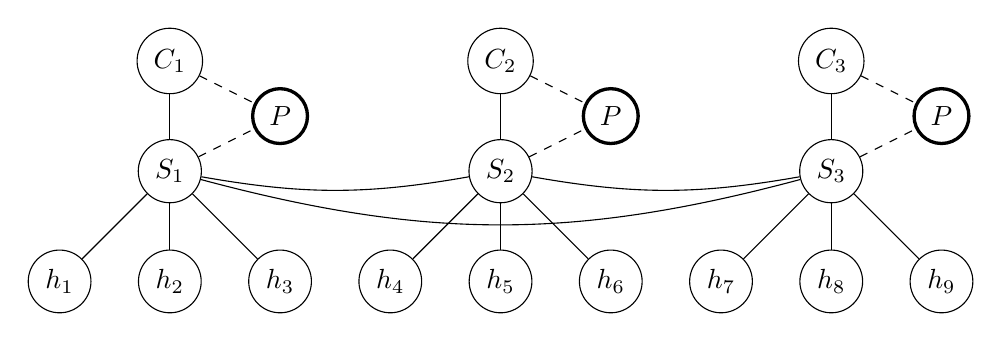
\begin{tikzpicture}[every node/.style={draw, circle},x=0.7cm,y=0.7cm]

    % For each switch ...
    \foreach \n in {1,2,3} {
      \pgfmathsetmacro\x{(\n-2)*6}
      \node (ctrl\n) at (\x ,  2) {$C_\n$};
      \node (S\n)    at (\x ,  0) {$S_\n$};

      \draw (S\n) -- (ctrl\n);

      % Paxos node
      \node [very thick] (P\n) at (\x + 2, 1) {$P$};
      \draw [dashed] (S\n) -- (P\n);
      \draw [dashed] (ctrl\n) -- (P\n);

      % For each host ...
      \foreach \h in {1,2,3} {
        \pgfmathsetmacro\pos{(\h - 2)*2}
        \pgfmathtruncatemacro\num{((\n - 1)*3) + int(\h)}

        % Host node
        \node (h\num) at (\x + \pos, -2) {$h_{\num}$};
        \draw (S\n) -- (h\num);
      }
    }

    % Links between switches
    \draw (S1) to[out=-10,in=190] (S2);
    \draw (S2) to[out=-10,in=190] (S3);
    \draw (S1) to[out=-15,in=195] (S3);

  \end{tikzpicture}
  \caption{Paxos ($P$) on the switches $S_1, S_2, S_3$ mitigates the need for special code on the servers.}
  \label{figure:paxos.on.switches}
\end{figure}

In figure \ref{figure:paxos.on.switches}, the switches themselves (and their
controllers\index{Paxos!controller}) enable
support for Paxos.\footnote{We have moved the servers to several switches
to indicate a distributed nature between the switches.
Paxos on a single switch would not be very useful, as that would be a single
point of failure and---after all---be the sole decision point for message
ordering.}
%
This should let the end-host services be oblivious to the fact that Paxos is
used to order the arrival of packets to them.

Besides, Paxos is now run at a much lower networking level\index{networking
layers} and at the point where switching is done---there will be less hops
for each packet.

Of course, there are pros and cons for each scenario.
When implementing Paxos, one can often take advantage of
the particular way each server operates. Sometimes one actually
\textit{needs} to know this to implement Paxos.  Therefore, an
implementation of Paxos in each server's code base would be beneficial.

Also, it means that we need to run code on the switches themselves. This
gives rise to a wide range of non-functional requirements for the code.
For instance, code that runs for too long must be
preempted\index{preemption} to let the switch smoothly handle other
requests. Not doing so may result in packet loss, high latency or
worse---complete incapacity to serve data. Besides, switches do not normally
have hardware capable of running \textit{generic} software fast. They
usually have highly optimized hardware to do some of the heavy-lifting.

On the other hand, in our scenario, we can \textit{potentially} add support
for replication through Paxos message ordering on services that does not
already support it.
%
We say ``potentially'', because it would only work for systems that are
deterministic on their input, meaning that by sending the same client
message to two service instances, they would perform the exact same action
and be left in the same state afterwards.
%
But many software services behave like this. For instance, one can imagine a
logging server that accepts client message and stores them on disk.
By duplicating each incoming client packet to all the logging instances,
they should all log the same messages---in the same order.
%
The same goes for many other type of services.  It all depends on the
details in how the services work, how complicated their message protocols
are and so on.  But one can certainly imagine this to work for key-value
stores, database servers, web-servers and so on.

We will not dive deeper into this matter.  Especially, we completely
disregard details concerning replies back to the clients: We silently
drop duplicated replies.  A deeper study would certainly take a closer
look at such situations.
%
Neither have we looked more at the situation when a switch goes down.
We have indicated fail-over links in the topologies, but have not
implemented such functionality.  For the part that concerns Paxos, such a
situation should start a new leader election.  If a switch comes back up
again, it should synchronize the state of its services with the others.
All of these are separate studies on their own, but we would like to note
that OpenFlow does have some support for monitoring link-status, and it
would be very interesting to make use of that in the face of failures.
%
Finally, we have not attempted to make an optimal design.  We concentrate
solely on the part of finding out if implementing Paxos on the switch-level
is \textit{possible} and if it could be \textit{useful}.

All in all, we believe this our limited design is a viable experiment that
should point the way toward practical merits.  After presenting our example
implementation in chapter \ref{chapter:implementation} we will discuss if
the system is viable in \ref{chapter:results}.
